%%%%% Despliegue

Para la fase dedespliegue, se explicar\'a como es el proceso para desplegar el sistema.

\section{Instalaci\'on de Foodprice}

Se debe realizar la clonaci\'on del paquete desde GitHub.
\\
\\
git clone \url{https://github.com/imcarlosguerrero/FoodpriceR}
\\
\\
Desde RStudio abrimos el archivo \textbf{FoodpriceR.Rproj} que pondr\'a a punto el entorno de trabajo sobre el cual se ejecutar\'a el paquete.

\begin{figure}[H]
    \centering
    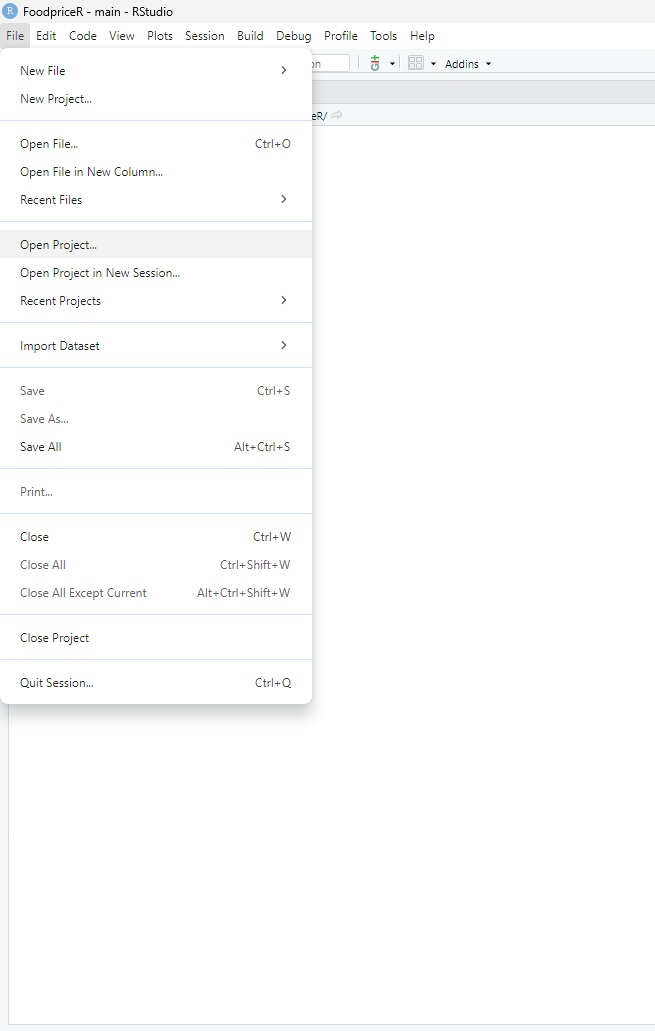
\includegraphics[height=10cm]{img/despliegue/despliegue4.jpeg}
    \caption{Despliegue del sistema}
    \label{fig:despliegue}
\end{figure}

\begin{figure}[H]
    \centering
    
\includegraphics[width=8cm]{img/despliegue/despliegue3.jpeg}
    \caption{Despliegue del sistema 2}
    \label{fig:despliegue2}
\end{figure}


En la consola de RStudio ejecutamos el siguiente comando.
\\
\\
\textbf{devtools::install("../FoodpriceR")}
\\
\\
Este instalar\'a el paquete Foodprice de manera local mientras nos encontramos dentro de la ruta de trabajo.
\\
\\
El paquete Foodprice requiere que en el entorno de trabajo se encuentren cargados los siguientes dataframes.

\begin{itemize}
    \item Mapeo\_Sipsa\_TCAC
    \item Mapeo\_Sipsa\_TCAC\_GABAS\_Grupos
    \item Mapeo\_Sipsa\_TCAC\_Carga\_2
    \item Primer\_Criterio\_Lista\_Alimentos
    \item intercambio\_gramos
    \item TCAC
\end{itemize}


Estos dataframes los podremos encontrar en la carpeta data que se encuentra dentro del proyecto y la cual podemos acceder desde el navegador de archivos de RStudio que se encuentra en la zona derecha del entorno de desarrollo.


\begin{figure}[H]
    \centering
    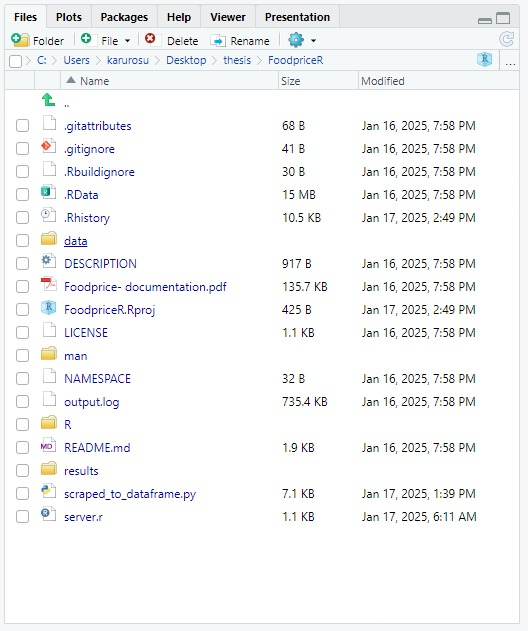
\includegraphics[height=10cm]{img/despliegue/despliegue2.jpeg}
    \caption{Despliegue del sistema 3}
    \label{fig:despliegue3}
\end{figure}


Una vez hayamos dado click sobre el dataframe que deseamos cargar, se abrir\'a una ventana emergente preguntando si queremos cargar dicho dataframe al entorno global, presionamos \textbf{``s\'i''}.

\begin{figure}[H]
    \centering
    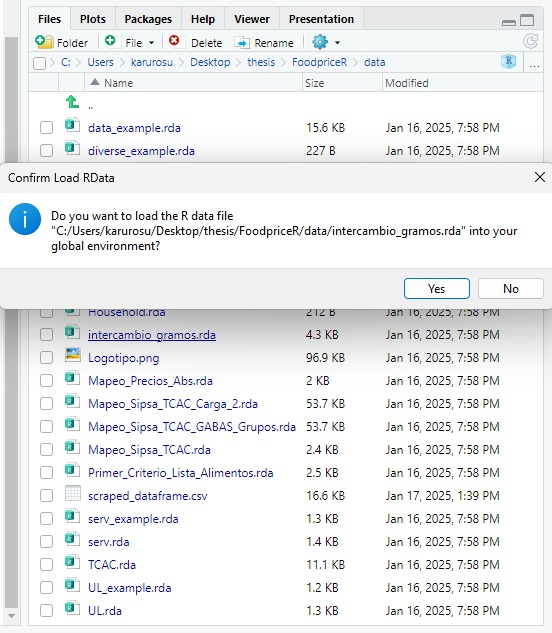
\includegraphics[height=10cm]{img/despliegue/despliegue.jpeg}
    \caption{Despliegue del sistema 4}
    \label{fig:despliegue4}
\end{figure}

y con esto ya tendremos cargado uno de los dataframe que el paquete Foodprice requiere para su funcionamiento, repitiendo este proceso por la cantidad de dataframes restantes, completaremos todos los requerimientos para poder comenzar a utilizar las funciones del paquete.